%==================================
\chapter{Architectural Description}
%==================================
This chapter introduces the architectural documents pertaining to our solution. The team followed the definition of software architecture defined by Len Bass, Paul Clements and Rick Kazman: ``The software architecture of a program or computing
system is the structure of structures of the system, which comprise software elements, the externally visible properties of those elements, and the relationships between them.''\cite[p.3]{Bass2003}

The purpose of this document is to describe our architecture in a structured way so that it can be used not only by the team, but also as an aid for other stakeholders who are trying to understand the system.

%------------------------------
\section{Architectural Drivers}
%------------------------------
This section is dedicated to the discussion of the architectural drivers.
The team has chosen Modifiability and Testability as the quality attributes for this \gls{utility}. 

The reason for using Modifiability is that the development team is not going to be the ones updating or maintaining the \gls{utility} after completing the project. It is therefore important that the code is easy to understand, well documented and easy to modify. This will make it easier for our customer to later modifiy or extend the \gls{utility}.

Testability is important since the \gls{utility} will be used for debugging by the customer.  Since it is not possible for the team to test the \glspl{dissector} in a real environment, it will be more important to focus on testing. This is to ensure that the final product is working correctly.

\subsection{Testability Tactics}
%-------------------------------
The goal of using testability tactics is making it easier to test the system after finishing an increment of the software development. 

\subsubsection{Specialize Access Routes/Interfaces}
Using a specialized testing interface makes it possible to specify values for a component independently from its normal execution. This will in turn make it possible to test parts of an unfinished module as well as making it easier to get a clear overview over what data is flowing through individual parts of the system. This is important for this project as the \gls{utility} must be able to run in a different environment than what the developers have access to. The testers must therefore be able to create input for each individual component of the system in order to ensure that it will work correctly with all kinds of input. 

\subsection{Modifiability Tactics}
%---------------------------------
The goal of using modifiability tactics is to make it easier to extend and modify the software during the development and after the completion of a working product.

\subsubsection{Anticipate Expected Changes}
By trying to anticipate expected changes it is possible to make it easier for modules to be extended with new functionality later. It also makes it easier for the developers to anticipate the different ranges of input the modules are able to process. This is important for this project as it is being developed incrementally, with new functionality and code added every sprint.

\subsubsection{Limit Possible Options}
By limiting the range of possible modifications to the system it becomes easier to generalize the structure of different modules. This will in turn make it easier to constrict the wide ranging effect of new modifications to the system, giving the developers a clearer view over what a given change will actually do to the system. This is important for this project as the developers have a limited time window to implement the \gls{utility}, making it important to be able to limit the scope of the \gls{utility} while still being able to add the functionality required by the customer.

\subsubsection{Generalizing Modules}
Generalizing the modules of a system makes it possible to reuse older modules when doing modifications to the system. The more general a module, the more likely it is that a needed change to the system can be implemented by just adjusting the input to the system, rather than having to modify existing or creating new modules.

\subsubsection{Restrict Communication Paths}
By restricting the number of modules that are able to collect data from a specific module, the less dependent the entire system becomes of that specific module. This makes it easier to swap out existing modules with new ones without having to make many widespread changes to the entire system. This is important for this project as the source code could change drastically after discovering new requirements in later sprints. By having a loose coupling we will minimize the amount of code that has to be rewritten after every sprint.

\subsubsection{Using Configuration Files}
By using configuration files, it is possible to change the behaviour of the system without having to do any changes to its code. It is very important that this system uses configuration files as this was a requirement from the customer, as well as making it more flexible for the end user.

\subsection{Business Requirements}
%---------------------------------
The following business requirements encompass the most important needs of the customer.
\begin{itemize}
\item The \gls{utility} must be delivered on time as it is not possible for the developers to continue the development after the deadline
\item The \gls{utility} should be able to create \glspl{dissector} for the \Gls{c}-\glspl{struct} in \gls{header} files used by Thales
\item The \gls{utility} should be able to create \glspl{dissector} that run on all of the platforms used by Thales and their customers
\item Developers at Thales should be able to use Gls{wireshark} with the generated \glspl{dissector} to display the values in \Gls{c}-\glspl{struct} passed through the system.
\end{itemize}

\subsection{Design Goals}
%------------------------
To help guide the design and the implementation we tried to follow these goals and guidelines:
\begin{itemize}
	\item Smart data structures and dumb code works better than the other way around\cite{Raymond1999}!
	\item Clear and clean separation of the front-end and the back-end so in the future other parsers can be used to generate \glspl{dissector}.
	\item Try to be pythonic, follow  PEP8 \footnote{Style Guide for Python Code: \url{http://www.python.org/dev/peps/pep-0008/}} and PEP20\footnote{The Zen of Python \url{http://www.python.org/dev/peps/pep-0020/}}.
	\item Now is better than never. Don't be afraid to write stupid or ugly code, we can always fix it later.
	\item The first version is never perfect, so don't wait until its perfect before you commit. Commit often!
\end{itemize}

%------------------------------
\section{Architectural Patterns}
%------------------------------
This section presents the different architectural patterns used in the \gls{utility}

\subsection{Pipe and Filter}
%---------------------------
The pipe and filter architectural pattern consists of a stream of data which in turn is processed sequentially by several filters, in such a fashion that the output of one filter becomes the input of the other. It is a very flexible, yet robust way of processing data, with support for adding more filters if needed for future applications and processes. As the \gls{utility} will only work on one piece of data that gradually changes, and is then converted into \Gls{lua}-code at the end, this seemed like a good and structured way of processing data early on, while still being able to add new functionality furhter down the line.

\begin{figure}[htb]
	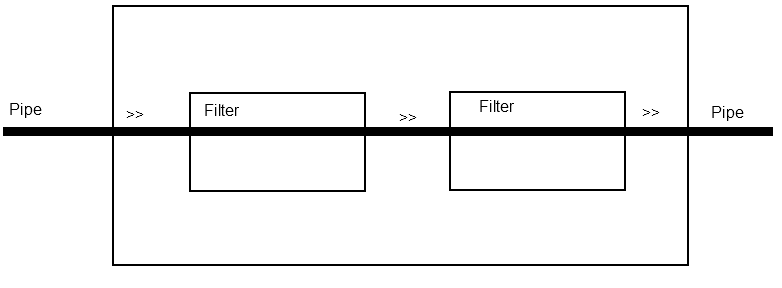
\includegraphics[width=\textwidth]{./planning/img/PipeAndFilter}
	\caption{Pipe and Filter Pattern\label{fig:pipefilter}}
\end{figure}


%----------------------------
\section{Architectural Views}
%----------------------------
This section describes three different views: Logival view, process view and deployment view.

\subsection{Logical View}
%------------------------
This view shown in \autoref{fig:logicalview}. Command line takes the arguments for \gls{header} file and configuration file as a string. The arguments are parsed in the command line \gls{parser}. Header file is sent to ''\Gls{c} \gls{preprocessor} \& \Gls{c} \gls{parser}'', the \Gls{c} \gls{header} file is loaded and parsed by the \Gls{c} \gls{parser}, whcih generates a parsing tree. Command line also call Configuration, which load the configuration file. The configuration will parse the configuration file and create configuation rules. The \Gls{lua} \gls{script} generator will generate a \Gls{lua} \gls{script} from the parsing tree and the config rules.

\begin{figure}[htb]
	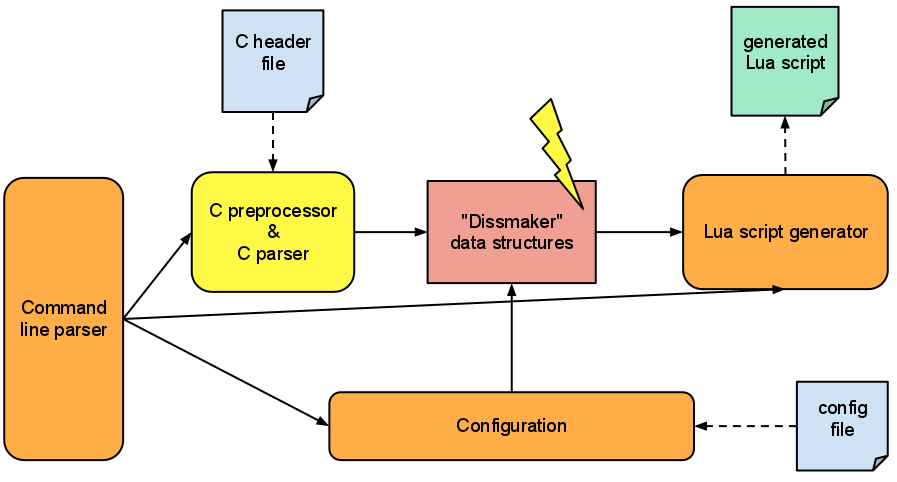
\includegraphics[width=\textwidth]{./planning/img/overall_design}
	\caption{Overall Architecture\label{fig:logicalview}}
\end{figure}


%---------------------
\subsection{Process View}
%---------------------
\autoref{fig:processview} shows the process view for our \gls{utility}. CSjark takes \gls{header} and config files as input and then uses the config and cparser to parse the files. CSjark then uses the cparser to find the \glspl{struct} in the \gls{header} file and then creates \glspl{dissector} for them. These \glspl{dissector} are then written to a file and CSjark then reports to the user by sending a message to the command line.

\begin{figure}[htb]
	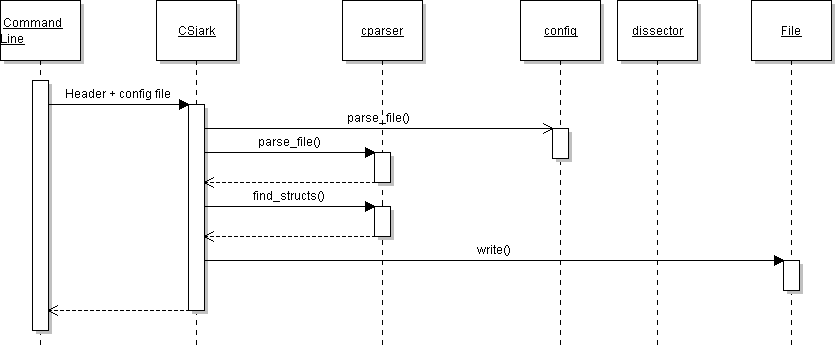
\includegraphics[width=\textwidth]{./planning/img/SequenceDiagram}
	\caption{Data flow during regular execution\label{fig:processview}}
\end{figure}


%------------------------
\subsection{Deployment View}
%------------------------
\autoref{fig:deployment} shows the deployment diagram for this project. CSjark 
takes \gls{header}-files and config-filess as input, and generates \Gls{lua} 
\glspl{dissector}. All these \glspl{dissector} are added as plugins to 
\Gls{wireshark}, to extend the functionality. \Gls{wireshark} will capture the 
data packet when Process A send data to Process B, the \Gls{lua} 
\glspl{dissector} is used to display these data packets correctly.

\begin{figure}[htb]
	\includegraphics[width = \textwidth]{./planning/img/Deployment}
	\caption{Deployment View\label{fig:deployment}}
\end{figure}


%--------------------------------
\section{Architectural Rationale}
%--------------------------------
The team decided to use the pipe and filter pattern as the architects felt that it was the only architectural pattern that would benefit the \gls{utility} without having to make it needlessly complex. The \gls{utility} was supposed to take \gls{header} files as input and then process the data from them several times, until the end result was a list of \glspl{struct} and \glspl{member} that could be used to make \glspl{dissector} for \Gls{wireshark}. This seemed like an excellent application to use the pipe and filter pattern with, as it would then be easy to add new filters to the \gls{header} file for future increments of the development cycle without having to rewrite what had already been implemented in previous sprints.

For the views the team decided to use a logical view, process view and deployment view. These views were chosen because the architects of the \gls{utility} felt that these views alone could represent the system sufficently without creating too much overhead for the readers of the document. The logical view supplies the reader with a more in depth view of what the system is comprised of, which is useful for developers who need to figure out the workings of the system. The process view also seemed important for the developers and the testers of the \gls{utility}, as it provides the reader with a more proper overview of the dataflow in the system. This makes it much easier to see which modules are run when, and to see which external calls dictate the modules' behaviour. Lastly a deployment view was chosen to make it more clear for the reader of the document what the \gls{utility} really produces as output and what other external applications it has to cooperate with. 

%------------------------------
\section{Changelog}
%------------------------------
 An architectural document should be thought of as a living document and treated as such. We wil therefore introduce the changes done to the architecture during each sprint in the following subsections.

\subsection{Sprint 1}
%---------------------
As we in sprint one was mostly concerned with getting the basic functionality in place, there were no changes done to the architecture.

\subsection{Sprint 2}
%----------------------
During the second sprint it became apparent that we needed to structure our code in a better and more organized way. If not, it would become very hard to add new functionality to the \gls{utility} in a straight forward and logical way. We therefore decided to introduce the layered architectural pattern (\ref{sec:Layered}), as it is often used to resolve issues just as the ones we faced in sprint 2. We also decided to add metrics for code coverage as a tactic for testability, in order to improve our unit tests

\subsubsection{Code Coverage}
By using a framework to see which parts and how much of the code is actually being run during the unit tests, it becomes easier to improve the quality of the unit tests. It could also be used as a checklist to see if the ones creating the unit tests have implemented some functionality that is currently not beng tested.


\subsection{Layered Architectural Pattern}
%-------------------------------------------------
\label{sec:Layered}
The layered architectural pattern is a pattern that involves grouping several different classes that all share the same dependencies. This grouping of classes is called a layer, and the layers are structured so that the classes inside each layer only depend on the classes of their own layer level, or inside an underlaying one. Structuring the code in this way helps delegating responsibilities to different parts of the system in a logical way, making the code easier to understand and easier to navigate through.

\autoref{fig:layered} shows how the layered architectural pattern is used in the \gls{utility}

\begin{figure}[htb]
	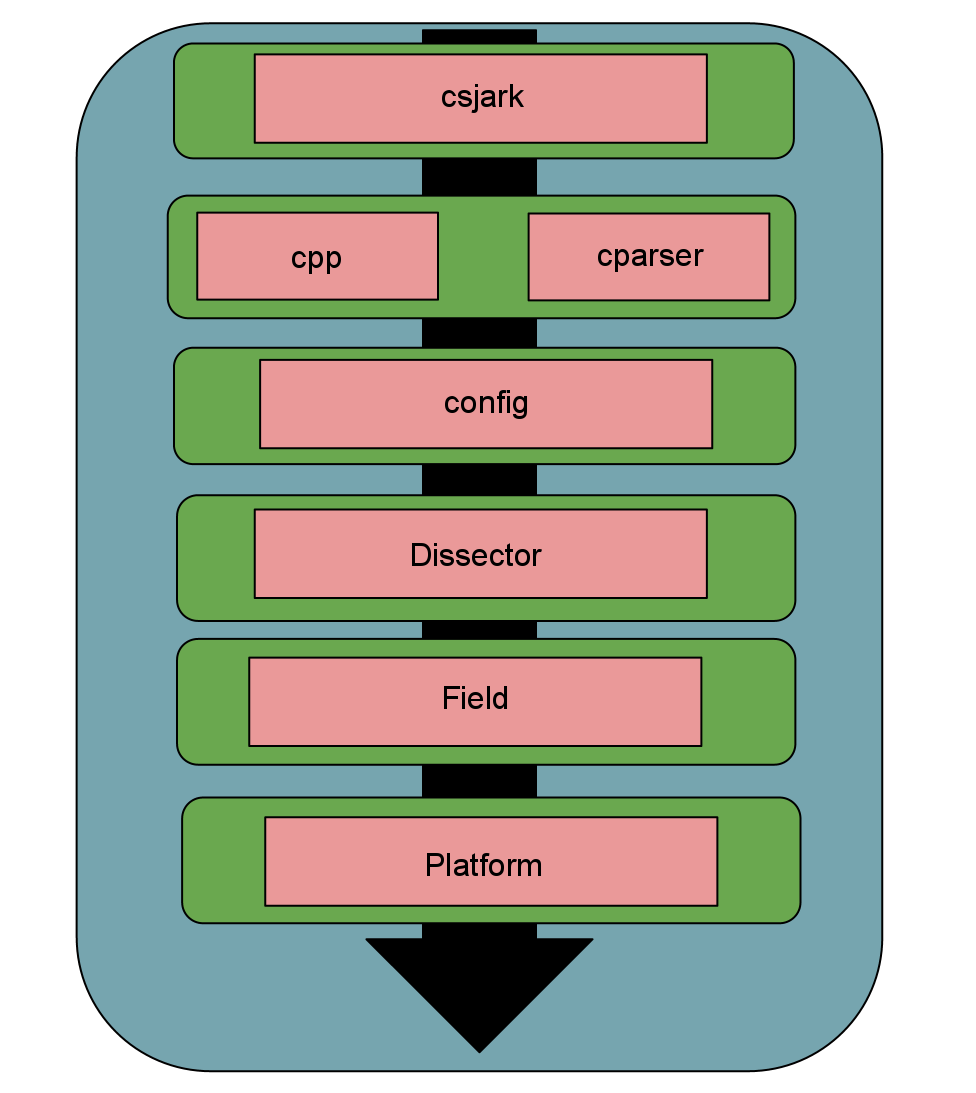
\includegraphics[width = \textwidth]{./planning/img/layered}
	\caption{Layered Architectural Pattern in the \gls{utility}\label{fig:layered}}
\end{figure}



\subsection{Sprint 3}
%------------------------
There were no additions or subtractions done to the architecture of the utility during sprint 3.

\subsection{Sprint 4}
%----------------------


